\documentclass{article}
\usepackage[hmargin=1in,vmargin=1.5in]{geometry}
\usepackage{amsmath}
\usepackage{amsfonts}
\usepackage{graphicx}
\usepackage{subcaption}
\usepackage{bm}
\renewcommand{\a}{\bm a}
\renewcommand{\c}{\bm c}
\newcommand{\p}{\bm p}
\newcommand{\q}{\bm q}
\newcommand{\1}{\bm 1}
\title{Homework 1}
\author{Xinyi Gu, Songchen Tan}
\date{\today}
\begin{document}
\maketitle
\section{}
\subsection*{(a)}

To deal with the absolute value in the objective function, We let vector $\a=\{a_0,\cdots,a_{T-1}\}=\p-\q$, where $p_t=\max(a_t,0)$ and $q_t=-\min(a_t,0)$; it is easy to verify that $a_t=p_t-q_t$ and $|a_t|=p_t+q_t$. Furthermore we denote $m=\max_{t\in\{0,\cdots,T-1\}}|a_t|$. Let $\c=(c_0,\cdots,c_{T-1})$ and $\1=(1,\cdots,1)$. The linear programming formulation is

minimize $m$, subject to

$$
\begin{cases}
    m >= (p_t + q_t), \quad 0\le t\le T-1\\
    \displaystyle
    \sum_{t=0}^{T-1}(p_t - q_t)=0\\
    \displaystyle
    \sum_{t=0}^{T-1}(T-t-1)(p_t - q_t)=d\\
    -\delta \le (p_{t-1} - q_{t-1})-(p_t - q_t) \le\delta, \quad 1\le t\le T-1\\
    \displaystyle
    \sum_{t=0}^{T-1}c_t(p_t+q_t)\le f
\end{cases}
$$

\subsection*{(b)}

The optimization gives $m\approx 0.0213$, and the $a, x, v$ are shown below.

\begin{figure}
    \centering
    \begin{subfigure}[b]{0.3\textwidth}
        \centering
        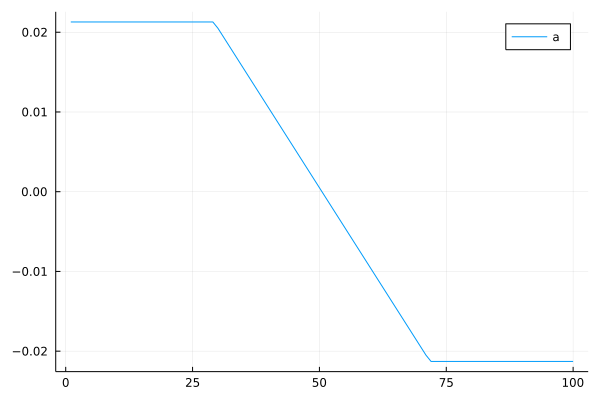
\includegraphics[width=\textwidth]{a.png}
        \caption{$a$}
    \end{subfigure}
    \hfill
    \begin{subfigure}[b]{0.3\textwidth}
        \centering
        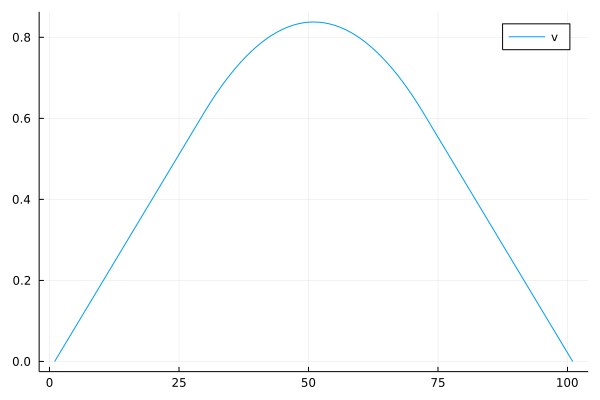
\includegraphics[width=\textwidth]{v.png}
        \caption{$v$}
    \end{subfigure}
    \hfill
    \begin{subfigure}[b]{0.3\textwidth}
        \centering
        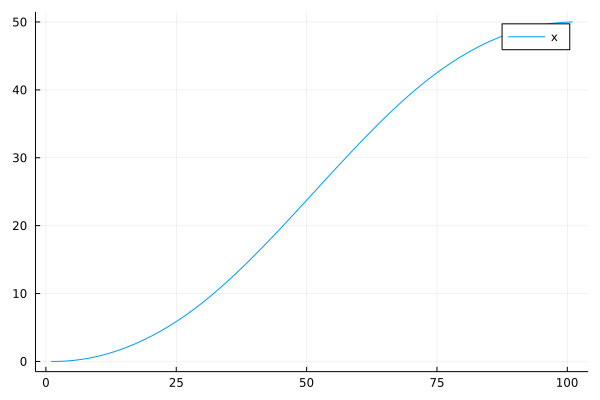
\includegraphics[width=\textwidth]{x.png}
        \caption{$x$}
    \end{subfigure}
       \caption{$a, x, v$ during the motion}
\end{figure}

\section{}

\subsection*{(a)} 

We have 

\begin{align*}
    \min \quad & c_1 x_1 + c_2 | x_2 -10| \\
    \text{subject to}\quad & c_3 | x_1 + 2 | + c_4 | x_2 | \le 5 
\end{align*}

Moving the objective into the constraints and making constraints with absolute valunes linear, we get

\begin{align*}
    \min \quad & t\\
    \text{subject to}\quad  z_1  & \geq  x_1 +2, \\
    z_1  & \geq -(x_1 + 2) \\
    z_2  & \geq  x_2 ,\\
    z_2  & \geq  -x_2\\
    c_3 z_1 + c_4 z_2 & \le 5, \\
    z_3  & \geq x_2 - 10 ,\\
    z_3  & \geq -(x_2 - 10)\\
    c_1 x_1 + c_2 z_3 & \le  t
\end{align*}

To formulate a linear programming problem, $c_1$ free, $c_2, c_3, c_4 \geq 0 $.

\subsection*{(b)} 

\begin{align*}
    f(x) & = \max{\{-x+1, \quad 0, \quad 2x - 4\}}\\
    c^{'}x + f(d^{'}x) & = c^{'}x + \max{\{-(d^{'}x) + 1, \quad 0, \quad 2(d^{'}x) - 4\}}
\end{align*}

Write max$\{\cdot\}$ as z and 3 constraints:

\[ z \geq - d^{'}x + 1, \quad z \geq 0, \quad z \geq 2d^{'}x - 4 \]

We get

\begin{align*}
    \min \quad & c^{'}x + z\\
    \text{subject to} \quad z & \geq - d^{'}x + 1,\\
    z & \geq 0,\\
    z & \geq 2d^{'}x - 4, \\
    Ax & \geq b
\end{align*}


\section{}

When $m\ge n$ this is trivial, so we consider $m < n$ only. For any $y\in\operatorname{ran}_+(A)$, consider the polyhedron

$$
C=\left\{x \in \mathbb{R}^{n} \mid y=A x, x \geq 0\right\}
$$

Assuming the rank of $A$ is $r\le m<n$, we can always select $r$ linearly independent rows such that, by row operations, they can eliminate other rows (including the corresponding elements in $y$). Therefore it suffices to prove the case $r=m$.

According to the corollary in class, every nonempty polyhedron in standard form has a BFS. $C$ is certainly nonempty since $y\in\textrm{ran}_+(A)$, so there exists a group of indices $B(1), \cdots, B(m)$ such that the matrix $B=(A_{B(1)}, \cdots, A_{B(m)})$ satisfies $B^{-1}y\ge 0$. This group of indices are the indices of coefficients required by the problem.


\section{}

\subsection*{(a)} 

True.

$n = m+1$ means that $P$ lives in an 1-D subspace, therefore every point in $P$ can be written as $x_0 + \lambda d$. This subspace is either a segment or a ray, so it can't have more than 2 extreme points.

\subsection*{(b)}
False.

Counter example: 
minimize $x_1$, subject to $x_1=1$ and $x_1,x_2\ge0$, optimal solution set is $\{(x_1,x_2)|x_1=1,x_2\geq0\}$ which is unbounded.

\subsection*{(c)} 
False.

Counter example: minimize $x_1+x_2$, subject to $x_1 +x_2= 1$, $x_1, x_2 \geq 0$. At a optimal solution $(0.5, 0.5)$, 2 (more than 1) variables are positive.

\subsection*{(d)} 
True.

Convex combination of any 2 (or more) solutions can be optimal.

\subsection*{(e)} 
False.

Same example as (b).

\subsection*{(f)} 
False.

Counter example: minimize $\max\{x_1-x_2,x_2-x_1\}$ subject to $x_1+x_2=1,x_1,x_2\ge0$. The optimal solution is $(0.5, 0.5)$.

\section{}

\subsection*{(a)}

We noticed that $\bar c_2<0$, therefore $\beta=0$ (or else it can be further optimized). We choose $(\alpha,\beta,\gamma,\delta,\eta)=(0, 0, 0, 0, 0)$.

\subsection*{(b)}

We need $d_j>0,\forall j\in N$, so we choose $j=1$ and $\alpha,\gamma,\delta <0$. We choose $(\alpha,\beta,\gamma,\delta,\eta)=(-1, 0, -1, -1, 0)$.

\subsection*{(c)}

We choose $j=2$ to be optimized, so we require $\beta>0$. We choose $(\alpha,\beta,\gamma,\delta,\eta)=(0, 3, 0, 1, 0)$.



\section{}

\subsection*{(a)}

Standard form:

\begin{align*}
    \min \quad  -2x_1 - x_2 & \\
    \text{subject to} \quad x_1 - x_2 + s_1 & = 2 \\
    x_1 + x_2 + s_2 & = 6 \\
    x_1, x_2, s_1, s_2 & \geq 0
\end{align*}

\[\begin{bmatrix}
    1 & -1 & 1 & 0 \\
    1 & 1 & 0 & 1
\end{bmatrix} \begin{bmatrix}
    x_1 & x_2 & s_1 & s_2
\end{bmatrix}^{T} = \begin{bmatrix}
    2 \\
    6
\end{bmatrix}
\]
Want ($x_1$, $x_2$) = (0, 0), pick $s_1$, $s_2$ as basis, 
B $ = \begin{bmatrix} 1 & 0 \\ 0 & 1 \end{bmatrix} $, 
BFS: $x^T = B ^{-1} b = $ (0, 0, 2, 6).

\subsection*{(b)}

Full tableau implementation:

start with BFS: x = (0, 0, 2, 6)'
B = [\boldsymbol{$A_3$}, \boldsymbol{$A_4$}]

\begin{tabular}{l|l|l|l|l|l|}
\cline{2-6}
&  & $x_1$ & $x_2$ & $s_1$ & $s_2$ \\ \cline{2-6} 
& 0 & -2 & -1 & 0 & 0 \\ \cline{2-6} 
 $s_1$ = & 2 & 1 & -1 & 1 & 0 \\ \cline{2-6} 
 $s_2$ = & 6 & 1 & 1 & 0 & 1\\ \cline{2-6} 
\end{tabular}
\\

$x_1$ and $x_2$ have negative reduced costs, pick $x_1$ to enter basis

\begin{tabular}{l|l|l|l|l|l|}
\cline{2-6}
&  & $x_1$ & $x_2$ & $s_1$ & $s_2$ \\ \cline{2-6} 
& 1 & 0 & 1 & 0 & 2 \\ \cline{2-6} 
 $x_1$ = & 6 & 1 & 1 & 0 & 1 \\ \cline{2-6} 
 $s_1$ = & -4 & 0 & -2 & 1 & -1\\ \cline{2-6} 
\end{tabular}
\\

$s_1 < $  0 here, infeasible solution, pick $s_2$

\begin{tabular}{l|l|l|l|l|l|}
\cline{2-6}
&  & $x_1$ & $x_2$ & $s_1$ & $s_2$ \\ \cline{2-6} 
& -3 & 0 & -3 & 2 & 0 \\ \cline{2-6} 
 $x_1$ = & 2 & 1 & -1 & 1 & 0 \\ \cline{2-6} 
 $s_2$ = & 4 & 0 & 2 & -1 & 1\\ \cline{2-6} 
\end{tabular}
\\
Then we have reduced costs of $x_2$ to be negative, pick $x_2$ to enter basis,

\begin{tabular}{l|l|l|l|l|l|}
\cline{2-6}
&  & $x_1$ & $x_2$ & $s_1$ & $s_2$ \\ \cline{2-6} 
& 10 & 0 & 0 & 0.5 & 1.5 \\ \cline{2-6} 
 $x_1$ = & 4 & 1 & 0 & 0.5 & 0.5 \\ \cline{2-6} 
 $x_2$ = & 2 & 0 & -1 & -0.5 & 0.5\\ \cline{2-6} 
\end{tabular}
\\
All the reduced costs in this tableau are nonnegative, representing an optimal solution at $x_1$ = 4 and $x_2$ = 2, $s_1$ = 0, $s_1$ = 0. In this solution, min $-2x_1 -x_2$ = $c^{'}_B x_B$ = -10


\end{document}





\\